\let\negmedspace\undefined
\let\negthickspace\undefined
\documentclass[journal]{IEEEtran}
\usepackage[a5paper, margin=10mm, onecolumn]{geometry}
%\usepackage{lmodern} % Ensure lmodern is loaded for pdflatex
\usepackage{tfrupee} % Include tfrupee package

\setlength{\headheight}{1cm} % Set the height of the header box
\setlength{\headsep}{0mm}     % Set the distance between the header box and the top of the text

\usepackage{gvv-book}
\usepackage{gvv}
\usepackage{cite}
\usepackage{amsmath,amssymb,amsfonts,amsthm}
\usepackage{algorithmic}
\usepackage{graphicx}
\usepackage{textcomp}
\usepackage{xcolor}
%\usepackage{txfonts}
\usepackage{listings}
\usepackage{enumitem}
\usepackage{mathtools}
\usepackage{gensymb}
\usepackage{comment}
\usepackage[breaklinks=true]{hyperref}
\usepackage{tkz-euclide} 
\usepackage{listings}
% \usepackage{gvv}                                        
\def\inputGnumericTable{}                                 
\usepackage[latin1]{inputenc}                                
\usepackage{color}                                            
\usepackage{array}                                            
\usepackage{longtable}                                       
\usepackage{calc}                                             
\usepackage{multirow}                                         
\usepackage{hhline}                                           
\usepackage{ifthen}                                           
\usepackage{lscape}
\usepackage{circuitikz}
\tikzstyle{block} = [rectangle, draw, fill=blue!20, 
    text width=4em, text centered, rounded corners, minimum height=3em]
\tikzstyle{sum} = [draw, fill=blue!10, circle, minimum size=1cm, node distance=1.5cm]
\tikzstyle{input} = [coordinate]
\tikzstyle{output} = [coordinate]


\begin{document}

\bibliographystyle{IEEEtran}
\vspace{3cm}

\title{5.2.16}
\author{EE25BTECH11013 - Bhargav}
\maketitle
{\let\newpage\relax\maketitle}

\renewcommand{\thefigure}{\theenumi}
\renewcommand{\thetable}{\theenumi}
\setlength{\intextsep}{10pt} % Space between text and floats

\numberwithin{equation}{enumi}
\numberwithin{figure}{enumi}
\renewcommand{\thetable}{\theenumi}

\textbf{Question}:\\
Solve the system of equations
\begin{align}
3x-5y=20
\end{align}
\begin{align}
6x-10y=40
\end{align}

\solution \\

The equation of line:
\begin{align}
\vec{n^T}\vec{x}=c
\end{align}

Line L:
\begin{align}
\myvec{3 & -5}\myvec{x \\ y}=20
\end{align}

Line K:
\begin{align}
\myvec{6 & -10}\myvec{x \\ y}=40
\end{align}

These can be combined and written in matrix form:
\begin{align}
\myvec{3 & -5 \\ 6 & -10}\myvec{x \\ y} = \myvec{20 \\ 40}
\end{align}

The following augmented matrix can be solved by gaussian elimination
\begin{align}
\augvec{2}{1}{3 & -5 & 20 \\ 6 & -10 & 40} \xleftrightarrow{R_2 \leftarrow R_2 - 2R_1} \augvec{2}{1}{3 & -5 & 20 \\ 0 & 0 & 0}
\end{align}

We end up with only one non -- zero row (Rank = 1)
\begin{align}
\myvec{3 & -5}\myvec{x \\ y} = 20
\end{align} \\ 


The general solution is 
\begin{align}
\myvec{x \\ y} = \myvec{t \\ \frac{3t-20}{5}} \quad t \in \mathbb{R}
\end{align}  \\

So there can be infinitely many solutions for this system of equations.


\begin{figure}[h!]
    \centering
    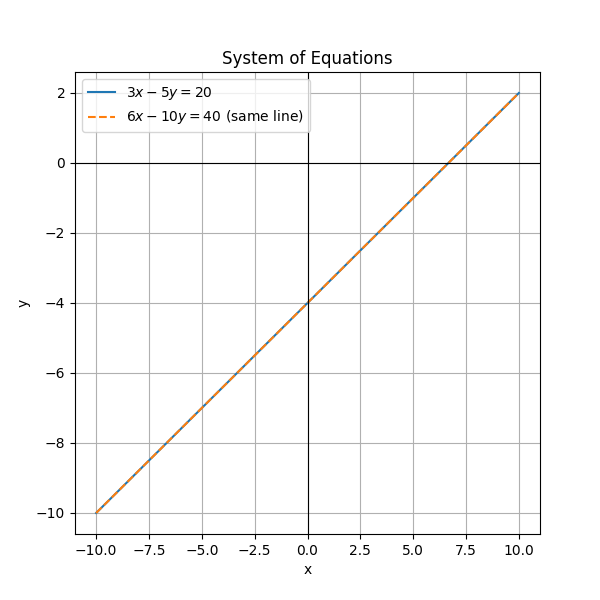
\includegraphics[height=0.5\textheight, keepaspectratio]{figs/Figure_1.png}
    \label{figure_1}
\end{figure}
\end{document}